\documentclass[border=8pt]{standalone}
% Shared TikZ style for every figure in "Post-training LLMs with RL" (see ../STYLE.md).
% Visual grammar follows the FME office-hours house style; the one accent colour is fern green.
% Compile with XeLaTeX, two passes (annotated equations remember node positions).
\usepackage{fontspec}
\setmainfont{Avenir Next}[BoldFont={Avenir Next Demi Bold}, ItalicFont={Avenir Next Italic}]
\setsansfont{Avenir Next}[BoldFont={Avenir Next Demi Bold}, ItalicFont={Avenir Next Italic}]
\renewcommand{\familydefault}{\sfdefault}
\hyphenpenalty=10000 \exhyphenpenalty=10000 % no hyphenation in notes and labels
\usepackage{amsmath,amssymb}
\usepackage{tikz}
\usetikzlibrary{arrows.meta,positioning,calc,fit,backgrounds,shapes.geometric,decorations.pathreplacing}

% ---------------- palette ----------------
\definecolor{ink}{HTML}{111111}
\definecolor{grey700}{HTML}{4A4F55}
\definecolor{grey500}{HTML}{6B7178}
\definecolor{grey400}{HTML}{8A9097}
\definecolor{grey300}{HTML}{D5D9DD}
\definecolor{grey100}{HTML}{F4F5F6}
\definecolor{fern}{HTML}{4F7942}       % the one accent: what the figure is about
\definecolor{ferndark}{HTML}{2F4A28}
\definecolor{fernlight}{HTML}{B5CFA8}
\definecolor{ferntint}{HTML}{EAF1E6}
% aliases used by older figure files
\colorlet{gray7}{grey700}\colorlet{gray5}{grey500}\colorlet{gray3}{grey300}\colorlet{gray1}{grey100}

% ---------------- visual grammar ----------------
\tikzset{
  every picture/.style={line cap=round, line join=round, color=ink},
  tensor/.style={draw=ink, line width=0.8pt, fill=white},
  param/.style={draw=grey700, line width=0.8pt, fill=grey100},
  op/.style={draw=grey500, line width=0.8pt, rounded corners=3pt, fill=white, inner sep=4pt, font=\small},
  accent/.style={draw=fern, line width=1.2pt},
  flow/.style={-{Stealth[length=5pt]}, line width=0.8pt, draw=grey700},
  flowa/.style={flow, draw=fern},
  tname/.style={font=\normalsize, text=ink},
  dims/.style={font=\footnotesize, text=grey500},
  note/.style={font=\footnotesize, text=grey700, align=left},
  accentnote/.style={font=\footnotesize, text=fern, align=left},
  lead/.style={draw=grey400, line width=0.5pt},
  stream/.style={draw=grey300, line width=5pt},
  block/.style={draw=grey500, line width=0.8pt, rounded corners=4pt, fill=white, align=center, font=\small, minimum height=0.8cm},
  blocka/.style={block, accent, fill=ferntint},
  frozen/.style={block, fill=grey100},
  plus/.style={circle, draw=grey700, line width=0.8pt, fill=white, inner sep=0pt, minimum size=0.42cm, font=\small},
  junction/.style={circle, fill=grey700, inner sep=0pt, minimum size=4pt},
  wire/.style={line width=0.8pt, draw=grey700},
}

% ---------------- numbered annotation system ----------------
%   markers on the drawing:  \mk{(x,y)}{1}   \mka{(x,y)}{2} (accent)
%   notes column:            \notesat{(x,y)}{width}  then  \note{1}{text}  /  \notea{2}{text}
%   symbols strip:           \symbols{$x$ & prompt \\ $y$ & response}
\tikzset{
  marker/.style={circle, fill=grey700, text=white, font=\footnotesize\bfseries, inner sep=0pt, minimum size=0.46cm},
  markera/.style={marker, fill=fern},
}
\newcommand{\mk}[2]{\node[marker] at #1 {#2}}
\newcommand{\mka}[2]{\node[markera] at #1 {#2}}
\newlength{\notewidth}
\newcommand{\notesat}[2]{%
  \node[inner sep=0pt, minimum size=0pt, anchor=north west] (note0) at #1 {};
  \setlength{\notewidth}{#2}\xdef\lastnote{note0}}
\newcommand{\note}[2]{%
  \node[font=\small, text=ink, align=left, text width=\notewidth, anchor=north west, inner sep=0pt] (note#1) at ($(\lastnote.south west)+(0.55cm,-0.32cm)$) {#2};
  \node[marker] at ($(note#1.north west)+(-0.30cm,-0.15cm)$) {#1};
  \path (note#1.south west) ++(-0.55cm,0) node[inner sep=0pt, minimum size=0pt] (note#1base) {};
  \xdef\lastnote{note#1base}}
\newcommand{\notea}[2]{%
  \node[font=\small, text=ferndark, align=left, text width=\notewidth, anchor=north west, inner sep=0pt] (note#1) at ($(\lastnote.south west)+(0.55cm,-0.32cm)$) {#2};
  \node[markera] at ($(note#1.north west)+(-0.30cm,-0.15cm)$) {#1};
  \path (note#1.south west) ++(-0.55cm,0) node[inner sep=0pt, minimum size=0pt] (note#1base) {};
  \xdef\lastnote{note#1base}}
\newcommand{\symbols}[1]{%
  \node[anchor=north west, inner sep=0pt, align=left, font=\small, text=grey700] (symbols)
    at ($(\lastnote.south west)+(0,-0.75cm)$)
    {\textcolor{grey400}{\scriptsize\bfseries SYMBOLS}\\[3pt]
     \begin{tabular}{@{}l@{\hspace{8pt}}l@{}}#1\end{tabular}};
  \draw[grey300, line width=0.5pt] ($(symbols.north west)+(0,0.18cm)$) -- ++(\notewidth+0.55cm,0);}

% ---------------- glyphs ----------------
\tikzset{
  expand/.style={draw=grey700, line width=0.8pt, fill=grey100, trapezium, trapezium stretches body,
                 trapezium left angle=64, trapezium right angle=64, shape border rotate=180,
                 minimum height=0.72cm, align=center, font=\small, inner xsep=2pt},
  contract/.style={expand, shape border rotate=0},
  silubox/.style={block, path picture={
      \begin{scope}[sharp corners, shift={($(path picture bounding box.west)+(0.45,-0.05)$)}, x=0.1cm, y=0.1cm]
        \draw[grey300, line width=0.4pt] (-3,0) -- (2.6,0);
        \draw[grey500, line width=1pt, domain=-3:2.4, samples=30] plot (\x, {\x/(1+exp(-\x))});
      \end{scope}}},
}

% ---------------- annotated equations (arrow + plain-language label per term) ----------------
% \tm{name}{math}: wrap one term of a formula in a named node. Put the formula node at (0,0)
% with anchor=base west, otherwise the remembered positions are offset.
\newcommand{\tm}[2]{\tikz[remember picture,baseline=(#1.base)]{\node[inner sep=1pt,outer sep=0pt] (#1) {$\displaystyle #2$};}}
\tikzset{
  lbl/.style   = {font=\large, text=ferndark, align=left, inner sep=2pt},
  lblg/.style  = {lbl, text=grey700},
  arr/.style   = {-{Stealth[length=8pt,width=6pt]}, line width=1.0pt, draw=fern, shorten >=3pt},
  arrg/.style  = {arr, draw=grey500},
  brc/.style   = {decorate, decoration={brace, mirror, amplitude=9pt, raise=5pt}, line width=1.4pt},
  % older diagram styles (kept for existing figures)
  blk/.style   = {draw=grey500, line width=0.9pt, rounded corners=6pt, fill=white, align=center, inner sep=7pt, minimum height=11mm, text=ink},
  blkf/.style  = {blk, draw=fern, line width=1.2pt, fill=ferntint},
  blkg/.style  = {blk, fill=grey100},
  ar/.style    = {-{Stealth[length=7pt,width=5pt]}, line width=1.0pt, draw=grey700},
  arf/.style   = {ar, draw=fern},
  capt/.style  = {font=\normalsize, text=grey500, align=center},
}

% ---------------- annotation protocol for equations ----------------
% The formula is one node named "eq" at (0,0), anchor=base west. Terms are wrapped with \tm.
% Labels sit in fixed rows ABOVE (a) or BELOW (b) the formula, tier 1 (near) or 2 (far), centred on
% their term (optional x-nudge), joined by a straight vertical leader with a dot on the term.
% No curved arrows, no diagonals. Tier-1 labels are at most two lines; tier-2 leaders pass between
% tier-1 labels. Sides l / r (outermost terms only): label beside the term, horizontal leader;
% the 4th argument is then a y-nudge.   \ann{term}{a|b|l|r}{1|2}{nudge}{text}    \anna{...} = accent (the slide's point)
\tikzset{
  annlbl/.style  = {font=\normalsize, text=grey700, align=center, inner sep=1.5pt},
  annlbla/.style = {annlbl, text=ferndark},
  annlead/.style = {draw=grey400, line width=0.6pt},
  annleada/.style= {draw=fern, line width=0.9pt},
}
\newcommand{\annrow}[2]{\ifnum#2=1 #1 0.55cm\else #1 1.95cm\fi}
\newcommand{\anngeneric}[7]{% #1 style-suffix, #2 term, #3 side, #4 tier, #5 nudge, #6 text, #7 lead style
  \if#3a
    \ifnum#4=1 \def\annoff{0.55cm}\else\def\annoff{1.95cm}\fi
    \node[annlbl#1, anchor=south] (ann-#2) at ($(#2.north |- eq.north)+(#5,\annoff)$) {#6};
    \draw[#7] ($(#2.north)+(0,0.13)$) -- (#2.north |- ann-#2.south);
    \fill[#7] ($(#2.north)+(0,0.13)$) circle (1.4pt);
  \else\if#3l
    \node[annlbl#1, anchor=east] (ann-#2) at ($(#2.west)+(-0.6cm,#5)$) {#6};
    \draw[#7] ($(#2.west)+(-0.13,0)$) -- (ann-#2.east |- {$(#2.west)+(0,0)$});
    \fill[#7] ($(#2.west)+(-0.13,0)$) circle (1.4pt);
  \else\if#3r
    \node[annlbl#1, anchor=west] (ann-#2) at ($(#2.east)+(0.6cm,#5)$) {#6};
    \draw[#7] ($(#2.east)+(0.13,0)$) -- (ann-#2.west |- {$(#2.east)+(0,0)$});
    \fill[#7] ($(#2.east)+(0.13,0)$) circle (1.4pt);
  \else
    \ifnum#4=1 \def\annoff{-0.55cm}\else\def\annoff{-1.95cm}\fi
    \node[annlbl#1, anchor=north] (ann-#2) at ($(#2.south |- eq.south)+(#5,\annoff)$) {#6};
    \draw[#7] ($(#2.south)+(0,-0.13)$) -- (#2.south |- ann-#2.north);
    \fill[#7] ($(#2.south)+(0,-0.13)$) circle (1.4pt);
  \fi\fi\fi}
\newcommand{\ann}[5]{\anngeneric{}{#1}{#2}{#3}{#4}{#5}{annlead}}
\newcommand{\anna}[5]{\anngeneric{a}{#1}{#2}{#3}{#4}{#5}{annleada}}

% ---------------- chart colours (validated with the dataviz palette checker, light surface) ----------
\definecolor{cvpr}{HTML}{4C8A35}   % CVPR series
\definecolor{acl}{HTML}{3B6EA8}    % ACL series
\usepackage{pgfplots}\pgfplotsset{compat=1.18}
\usepgfplotslibrary{groupplots}
\pgfplotsset{
  surveyaxis/.style={axis lines=left, axis line style={grey400, line width=0.6pt, -}, tick style={grey400},
    tick label style={font=\footnotesize, text=grey700}, label style={font=\small, text=grey700},
    ymajorgrids, grid style={grey300, line width=0.3pt}, enlarge x limits=0.12, clip=false},
}

\begin{document}
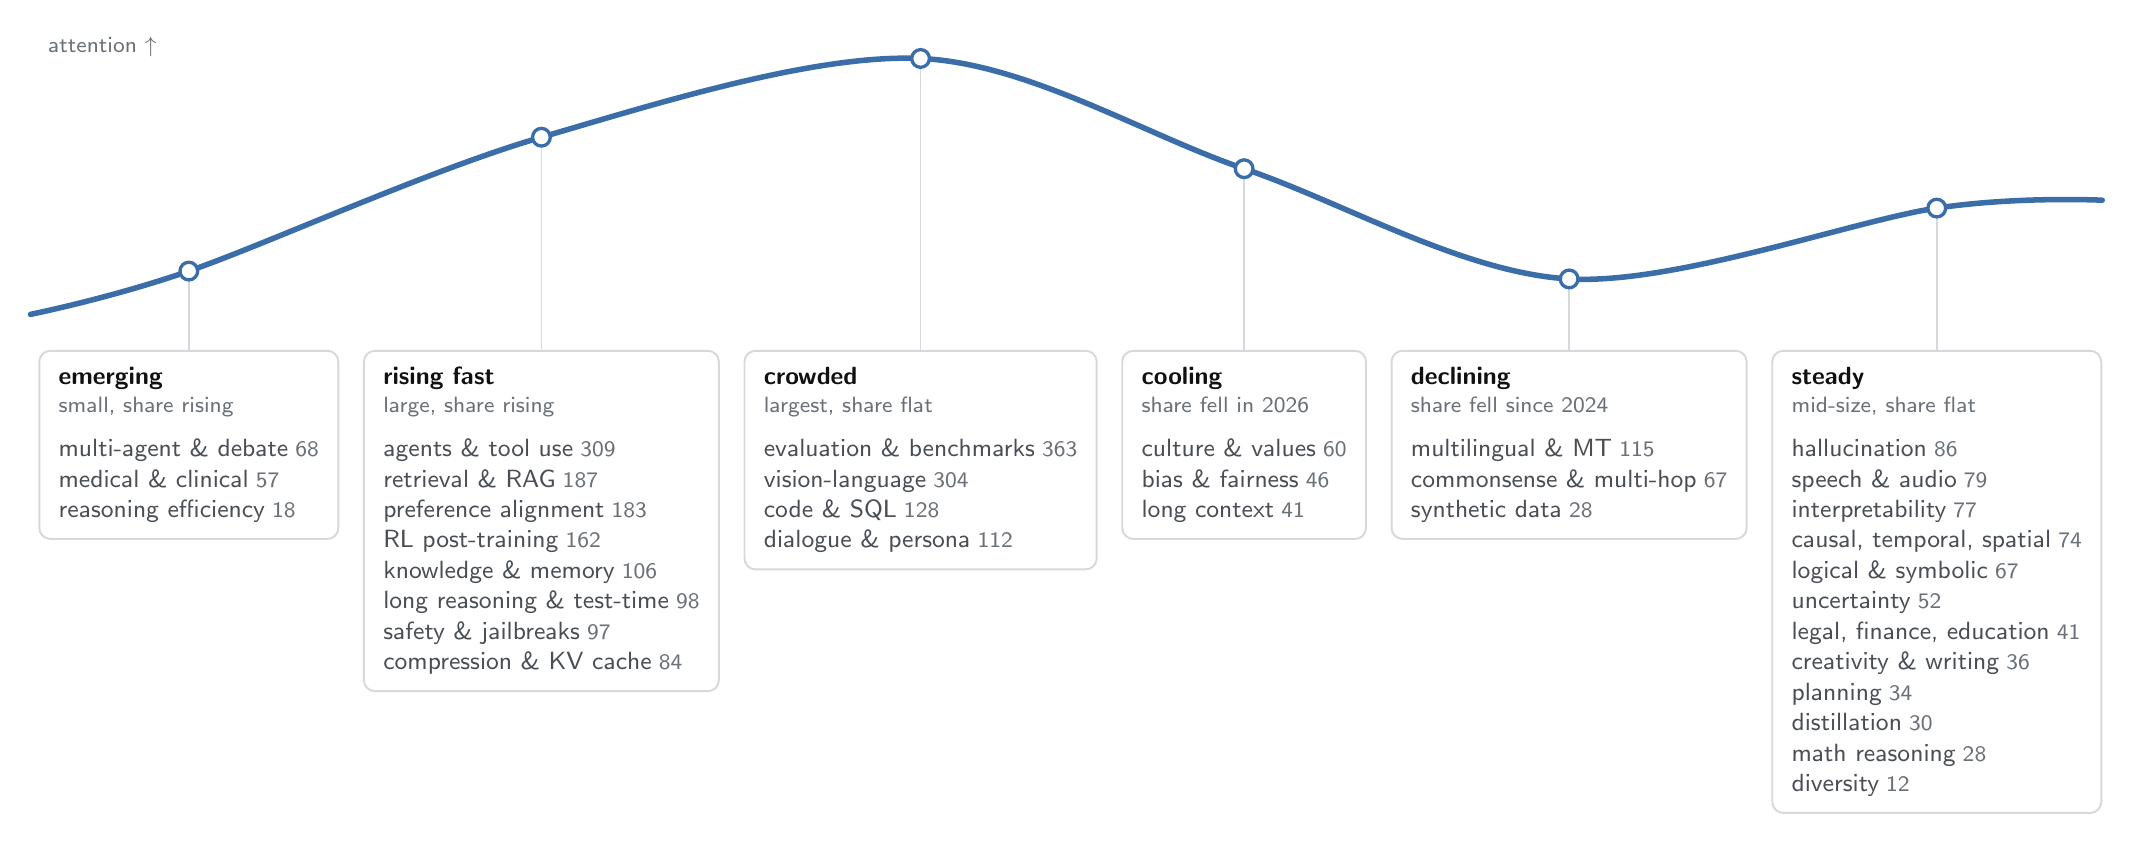
\begin{tikzpicture}[font=\small, card/.style={draw=grey300, line width=0.7pt, rounded corners=4pt, fill=white, inner xsep=7pt, inner ysep=6pt, anchor=north west, align=left}]
\node[card] (c0) at (0,0) {\textbf{\color{ink}emerging}\\[-1pt]{\footnotesize\color{grey500}small, share rising}\\[5pt]{\color{grey700}multi-agent \& debate}\;{\footnotesize\color{grey500}68}\\{\color{grey700}medical \& clinical}\;{\footnotesize\color{grey500}57}\\{\color{grey700}reasoning efficiency}\;{\footnotesize\color{grey500}18}};
\coordinate (s0) at ([yshift=1.0cm]c0.north);
\node[card] (c1) at ([xshift=0.3cm]c0.north east) {\textbf{\color{ink}rising fast}\\[-1pt]{\footnotesize\color{grey500}large, share rising}\\[5pt]{\color{grey700}agents \& tool use}\;{\footnotesize\color{grey500}309}\\{\color{grey700}retrieval \& RAG}\;{\footnotesize\color{grey500}187}\\{\color{grey700}preference alignment}\;{\footnotesize\color{grey500}183}\\{\color{grey700}RL post-training}\;{\footnotesize\color{grey500}162}\\{\color{grey700}knowledge \& memory}\;{\footnotesize\color{grey500}106}\\{\color{grey700}long reasoning \& test-time}\;{\footnotesize\color{grey500}98}\\{\color{grey700}safety \& jailbreaks}\;{\footnotesize\color{grey500}97}\\{\color{grey700}compression \& KV cache}\;{\footnotesize\color{grey500}84}};
\coordinate (s1) at ([yshift=2.7cm]c1.north);
\node[card] (c2) at ([xshift=0.3cm]c1.north east) {\textbf{\color{ink}crowded}\\[-1pt]{\footnotesize\color{grey500}largest, share flat}\\[5pt]{\color{grey700}evaluation \& benchmarks}\;{\footnotesize\color{grey500}363}\\{\color{grey700}vision-language}\;{\footnotesize\color{grey500}304}\\{\color{grey700}code \& SQL}\;{\footnotesize\color{grey500}128}\\{\color{grey700}dialogue \& persona}\;{\footnotesize\color{grey500}112}};
\coordinate (s2) at ([yshift=3.7cm]c2.north);
\node[card] (c3) at ([xshift=0.3cm]c2.north east) {\textbf{\color{ink}cooling}\\[-1pt]{\footnotesize\color{grey500}share fell in 2026}\\[5pt]{\color{grey700}culture \& values}\;{\footnotesize\color{grey500}60}\\{\color{grey700}bias \& fairness}\;{\footnotesize\color{grey500}46}\\{\color{grey700}long context}\;{\footnotesize\color{grey500}41}};
\coordinate (s3) at ([yshift=2.3cm]c3.north);
\node[card] (c4) at ([xshift=0.3cm]c3.north east) {\textbf{\color{ink}declining}\\[-1pt]{\footnotesize\color{grey500}share fell since 2024}\\[5pt]{\color{grey700}multilingual \& MT}\;{\footnotesize\color{grey500}115}\\{\color{grey700}commonsense \& multi-hop}\;{\footnotesize\color{grey500}67}\\{\color{grey700}synthetic data}\;{\footnotesize\color{grey500}28}};
\coordinate (s4) at ([yshift=0.9cm]c4.north);
\node[card] (c5) at ([xshift=0.3cm]c4.north east) {\textbf{\color{ink}steady}\\[-1pt]{\footnotesize\color{grey500}mid-size, share flat}\\[5pt]{\color{grey700}hallucination}\;{\footnotesize\color{grey500}86}\\{\color{grey700}speech \& audio}\;{\footnotesize\color{grey500}79}\\{\color{grey700}interpretability}\;{\footnotesize\color{grey500}77}\\{\color{grey700}causal, temporal, spatial}\;{\footnotesize\color{grey500}74}\\{\color{grey700}logical \& symbolic}\;{\footnotesize\color{grey500}67}\\{\color{grey700}uncertainty}\;{\footnotesize\color{grey500}52}\\{\color{grey700}legal, finance, education}\;{\footnotesize\color{grey500}41}\\{\color{grey700}creativity \& writing}\;{\footnotesize\color{grey500}36}\\{\color{grey700}planning}\;{\footnotesize\color{grey500}34}\\{\color{grey700}distillation}\;{\footnotesize\color{grey500}30}\\{\color{grey700}math reasoning}\;{\footnotesize\color{grey500}28}\\{\color{grey700}diversity}\;{\footnotesize\color{grey500}12}};
\coordinate (s5) at ([yshift=1.8cm]c5.north);
\coordinate (s-) at ([xshift=-0.1cm, yshift=0.45cm]c0.north west);
\coordinate (s+) at ([yshift=1.9cm]c5.north east);
\draw[acl, line width=2pt] plot[smooth, tension=0.55] coordinates {(s-) (s0) (s1) (s2) (s3) (s4) (s5) (s+)};
\draw[grey300, line width=0.6pt] ([yshift=-3.2pt]s0) -- (c0.north);
\fill[white, draw=acl, line width=1.2pt] (s0) circle (3.2pt);
\draw[grey300, line width=0.6pt] ([yshift=-3.2pt]s1) -- (c1.north);
\fill[white, draw=acl, line width=1.2pt] (s1) circle (3.2pt);
\draw[grey300, line width=0.6pt] ([yshift=-3.2pt]s2) -- (c2.north);
\fill[white, draw=acl, line width=1.2pt] (s2) circle (3.2pt);
\draw[grey300, line width=0.6pt] ([yshift=-3.2pt]s3) -- (c3.north);
\fill[white, draw=acl, line width=1.2pt] (s3) circle (3.2pt);
\draw[grey300, line width=0.6pt] ([yshift=-3.2pt]s4) -- (c4.north);
\fill[white, draw=acl, line width=1.2pt] (s4) circle (3.2pt);
\draw[grey300, line width=0.6pt] ([yshift=-3.2pt]s5) -- (c5.north);
\fill[white, draw=acl, line width=1.2pt] (s5) circle (3.2pt);
\node[anchor=south west, font=\footnotesize, text=grey500] at ([yshift=3.6cm]c0.north west) {attention $\uparrow$};
\end{tikzpicture}
\end{document}
